\chapter{Introduction}
\section{Motivation}
Description of Status Quo\newline
What is the Problem? AutoWDS does not scale/work well \newline
What do we want? Make AutoWDS Useful/scalable/work again \newline
Why are we doing this? Provide a system to easily deploy of a set of accesspoints for creating a wireless lan infrastructure \newline
How do we want to do/solve this? Using multiple Channels \newline
Using Redundant Paths Using a better Network Topology \newline
What problems could arise? Finding a good network-topology/CAA tricky \newline
How are we planing on dealing with these problems? \newline
What (data) do we need to solve the Problem? Central Inter-AP SNR \newline

\section{Structure of Thesis}
In the first Chapter we do this and this, in the second, this ...

Below This examples:

\begin{listing}[t]
\begin{lstlisting}
#include <stdio.h>

int main(void)
{
	printf("Hello, World\n");

	return 0;
}
\end{lstlisting}
\caption{A simple code example.}
\label{lst:example}
\end{listing}

\begin{figure}[t]
\centering
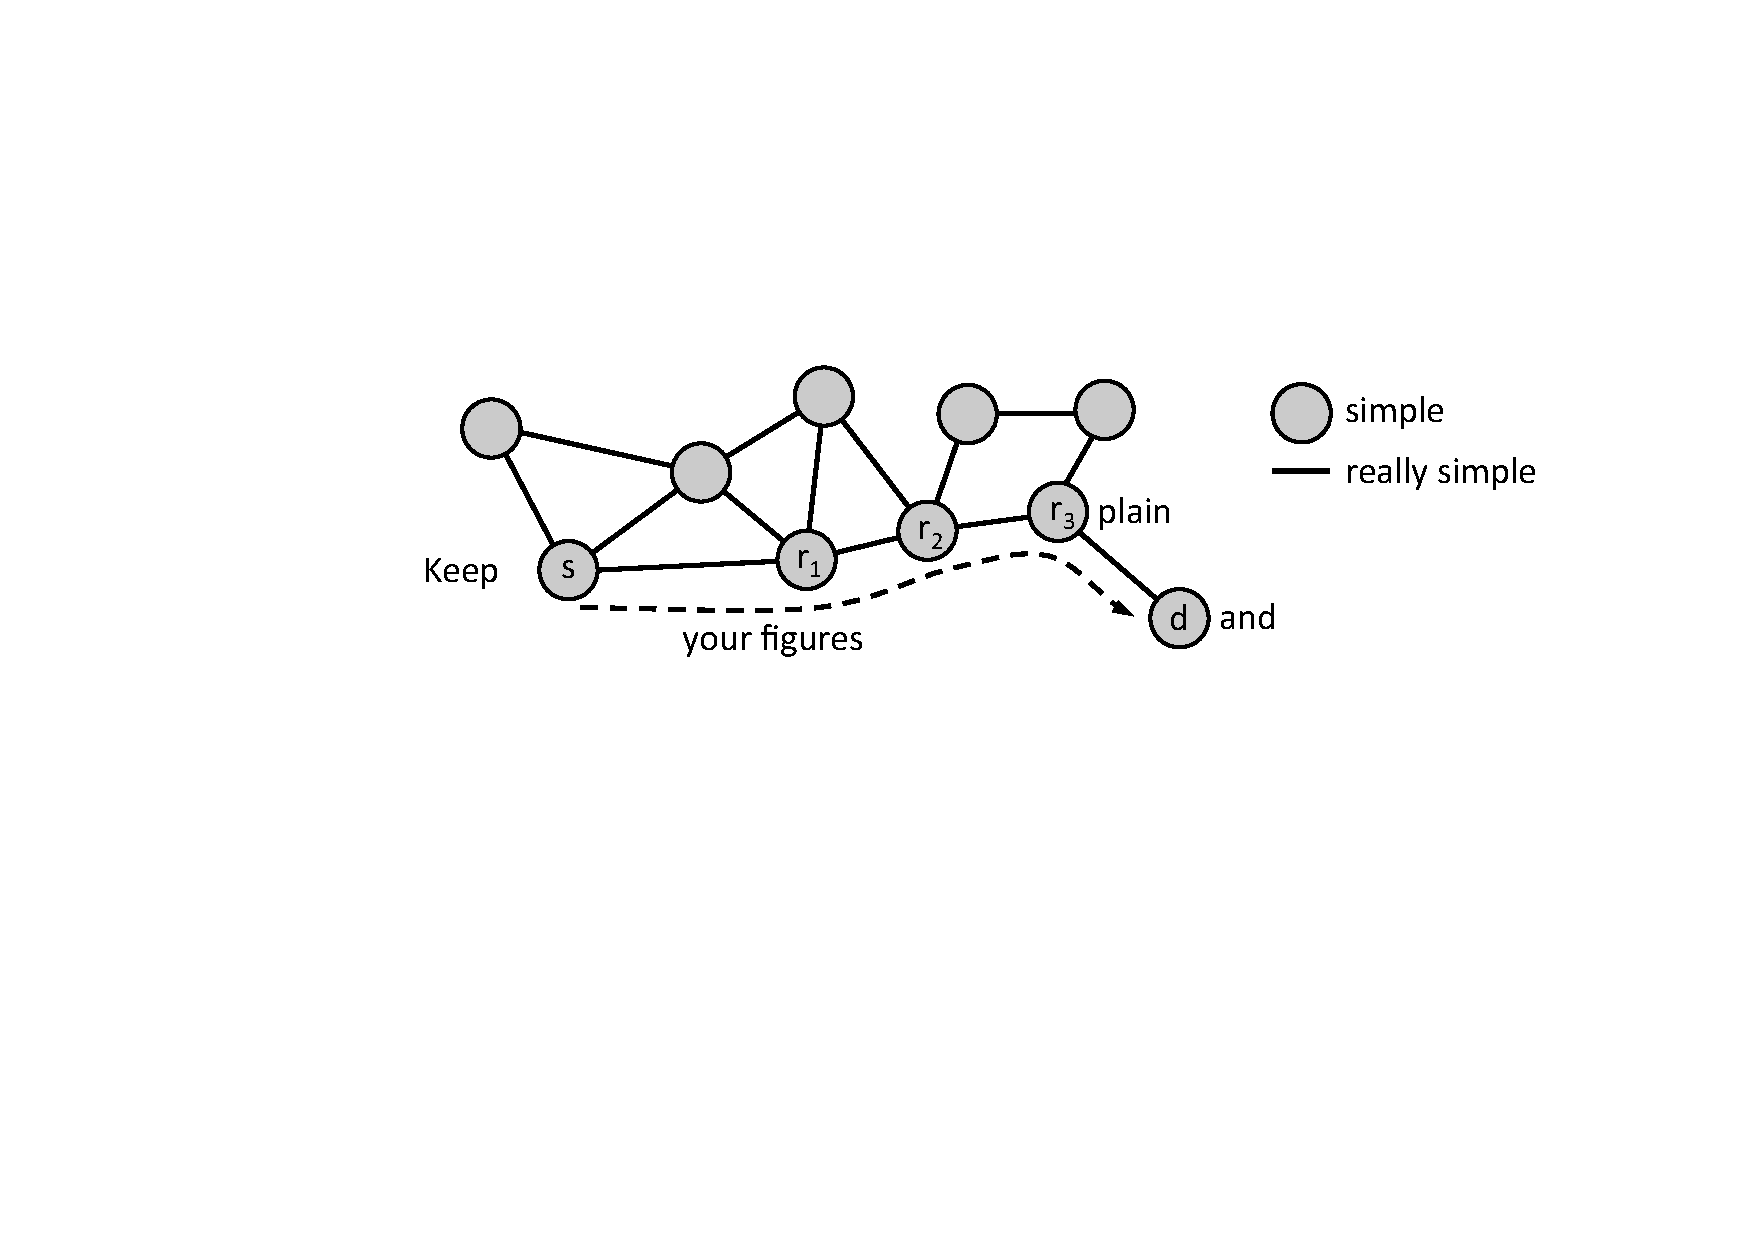
\includegraphics[width=1\columnwidth]{figures/example}
\caption{An example of an awesome image!}
\label{fig:example}
\end{figure} 

\begin{description}
\item[Ut ac ipsum:]
Ut ac ipsum at velit malesuada tincidunt ornare at sapien. Aenean at dui dolor. Pellentesque sit amet fermentum lorem. Nullam pulvinar diam eget diam hendrerit condimentum. Duis fermentum vulputate ante, a egestas mauris vehicula at. Quisque convallis vestibulum fermentum.

\item[Aenean lacinia elementum:]
Aliquam sed ante id velit ultricies condimentum. Aenean lacinia elementum lacus sit amet luctus. Vestibulum consequat nibh et tortor laoreet sit amet vehicula orci venenatis. Suspendisse enim velit, hendrerit quis vestibulum sit amet, tincidunt sit amet odio.

\item[Phasellus id:]
Nullam ut est lacinia est auctor consectetur faucibus nec tellus. Phasellus id tincidunt risus. Nulla volutpat quam vel diam vehicula in egestas ligula laoreet. 

\end{description}

\begin{table}[b]
\caption{Tables should look like this (save for the last row). If you know LaTeX better than me, feel free to improve the way of producing these tables.}
\begin{tabularx}{\linewidth}{|l|X|X|}
\hline
\rowcolor{slightgray}
\T Tables	&have gray  &headlines\\
\hline
\cellcolor{slightgray}\T and gray &labels \B&, too.\\
\hline
\cellcolor{slightgray}\T T &and B& are used for spacing\B\\
\hline
\cellcolor{slightgray} without T & and B& the cells are too small\B\\
\hline 
\end{tabularx}
\label{tab:example}
\end{table}

%These are reference and cite examples. See Figure~\ref{fig:example}, Table~\ref{tab:example}, and Listing~\ref{lst:example}. Cite early and often~\cite{exampleentry} is a good rule of thumb.
